\section{Exact examples and a regularity obstruction}\label{sec:examples}
These examples have \(X=[-1,1]\), \(m=1\), \(q_0=1\), and \(b^*=0\).
They permit direct integration, independently of the coefficient formulas.

\subsection{An asymmetric two-switch example}
Let
\[
 q_1(x)=(x^2-\tfrac14)(1+\beta x),\qquad |\beta|<1,\qquad f=\tfrac18 .
\]
The zeros are \(\pm1/2\), and the sign has zero mean.
For small \(a\), exact mean balance puts the two centers at
\(c_\pm=d\pm1/2\). Their individual balance equations coincide:
\[
 2d+3\beta d^2+\beta a^2=0 .
\]
The solution near zero is
\(d=-\beta a^2/2-3\beta^3a^4/8+O(a^6)\).
Integration of the resulting profile gives
\[
 S(a)=\tfrac12-\tfrac23a^2+\tfrac{\beta^2}{2}a^4+O(a^6).
\]
In particular,
\begin{equation}\label{eq:exampleone}
 \delta_0=\tfrac14,\qquad C_2=\tfrac1{48},\qquad
 C_4=\frac{16/3-\beta^2}{1024}.
\end{equation}
As an exact arithmetic check, for \(\beta=1/4\),
\[
 G=\frac{256}{63},\quad B=\frac{244}{189},\quad
 R=\frac{134}{567},\quad P=\frac{3721}{18144},\quad
 \Xi=\frac1{32},\quad C_4=\frac{253}{49152}.
\]
The cancellation producing \(\Xi\) is substantial enough that retaining
the moment correction matters.

\subsection{A negative fourth coefficient}
Let \(q_1(x)=x-3x^3+9x^5\) and \(f=5/8\).
Since \(q_1=x\{(3x^2-1/2)^2+3/4\}\), there is a single simple switch
at zero. Odd symmetry gives the balanced center exactly.
The supported moment is
\[
 S(a)=\tfrac52-\tfrac13a^2+\tfrac3{10}a^4-\tfrac37a^6.
\]
Inverting with \(a=A/M\) gives
\begin{equation}\label{eq:examplenegative}
 \delta(M)=\tfrac14+\frac1{480M^2}
                        -\frac1{15360M^4}+O(M^{-6}).
\end{equation}
The underlying weight here is the positive constant \(1\), so it cannot
enforce positivity of \(C_4\).

\subsection{Why twice continuous differentiability is insufficient}
Let \(q_1(x)=x+\sgn(x)|x|^{5/2}\) and \(f=11/28\).
This function is \(C^2\), with a simple zero at zero, but is not \(C^3\).
The exact ramp moment is
\[
 S(a)=\frac{11}{7}-\frac{a^2}{3}-\frac{8a^{7/2}}{63}.
\]
Consequently,
\begin{equation}\label{eq:regularityexample}
 \delta(M)=\tfrac14+\frac7{2112M^2}
                         +\frac1{6336M^{7/2}}+O(M^{-4}).
\end{equation}
Thus a finite coefficient in a remainder of the form
\(C_4M^{-4}+o(M^{-4})\) after the second-order term does not exist.
This is consistent with the \(o(M^{-3})\) conclusion under \(C^2\).

\begin{figure}[tb]
 \centering
 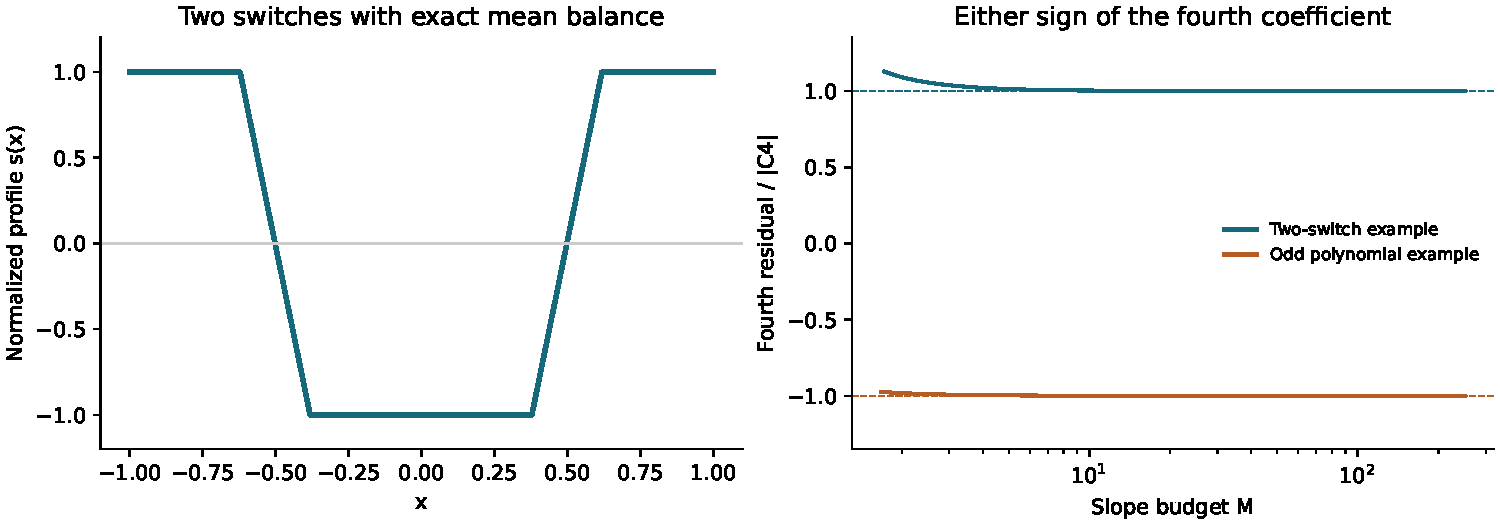
\includegraphics[width=.96\linewidth]{figures/examples.pdf}
 \caption{Left: the unique normalized optimizer in the two-switch
 example with \(\beta=1/4\) at ramp half-width \(a=0.12\), computed
 from its exact balance equation. Right: the scaled residual
 \(M^4(\delta(M)-\delta_0-C_2/M^2)/|C_4|\) for the first two examples,
 with the analytic limits \(+1\) and \(-1\) as dashed lines.
 The curves are high-precision evaluations of their explicit scalar
 equations, not interval certificates.}
 \label{fig:examples}
\end{figure}
